\section{Related Work}
\label{sec:related-work}

\subsection{Data-Adaptive Compression in Database Systems}
\label{sec:related-work:database}

Compression has long been integrated into database and data management systems to reduce storage and data movement costs~\cite{li1987compression}. In modern data-management platforms, BtrBlocks~\cite{kuschewski2023btrblocks} and ALP~\cite{afroozeh2023alp} provide lossless compression for columnar storage in data lakes and floating-point columns in analytical systems, respectively. ASZ also targets data-management systems, providing error-bounded lossy compression for multidimensional scientific fields.

\subsection{Error-Bounded Lossy Compression}
\label{sec:related-work:compression}

Error-bounded lossy compression supports scientific data management by reducing storage requirements and data movement through I/O and network transfers while controlling reconstruction error~\cite{cappello2019use,di2025survey}.

Prediction-based compressors such as SZ3~\cite{zhao2021optimizing,liang2022sz3} and QoZ~\cite{liu2022dynamic,liu2024high} often predict each data value as a weighted combination of neighboring values. They then quantize the prediction error and encode the resulting quantization-bin index. ASZ belongs to this class and follows the SZ pipeline used by SZ3 and QoZ, reviewed in Sections~\ref{sec:background:pipeline}--\ref{sec:background:configuration-granularity}.

Transform-based compressors such as ZFP~\cite{lindstrom2014fixed}, SPERR~\cite{li2023lossy}, and MGARD~\cite{gong2023mgard} use block transforms, wavelets, and multilevel decompositions, respectively.

\subsection{Commonly Tuned Dimensions}
\label{sec:related-work:dimensions}

We first summarize the configurations commonly tuned by existing prediction-based compressors.

\begin{figure}[!t]
\centering
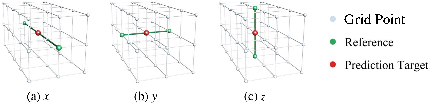
\includegraphics[width=\linewidth]{revised-fig/stencils-in-3-directions.pdf}
\caption{The same two-reference linear-interpolation stencil aligned with the three axes of a three-dimensional field.}
\label{fig:related-work:stencil-axes}
\vspace{-0.6\baselineskip}
\end{figure}

\begin{enumerate}
\item \emph{Prediction Stencils.}\par\noindent\mbox{\hspace{1em}}A prediction stencil is a pattern of reference points around a target. Taking the linear-interpolation stencil shown in Fig.~\ref{fig:related-work:stencil-axes} as an example, the stencil uses two references equidistant from the target along the selected prediction axis, and the reference spacing sets their distance from the target. The predictors in the three subfigures use different references and can produce different predicted values, but they share the same prediction stencil.

\noindent\mbox{\hspace{1em}}Many compressors tune prediction stencils. For example, SZauto~\cite{zhao2020significantly} tunes the range of reference points used by Lorenzo prediction. SZ3 considers Lorenzo prediction as well as linear and cubic interpolation stencils. QoZ 2.0~\cite{liu2024high} and GPU-based cuSZ-Hi~\cite{wu2025boosting} may further divide a prediction round into two passes, allowing second-pass targets to use values reconstructed in the first pass as additional references. The resulting variants include a six-reference one-dimensional cubic stencil and stencils that draw references from multiple dimensions.

\item \emph{Prediction Axes.}\par\noindent\mbox{\hspace{1em}}Prediction axes determine how a stencil is oriented relative to the data grid. Compressors such as SZ3, QoZ, cuSZ-Hi, and CliZ~\cite{jian2024cliz} tune these axes. QoZ and CliZ can also avoid prediction along less smooth axes throughout the compression procedure.

\item \emph{Prediction Coefficients.}\par\noindent\mbox{\hspace{1em}}Prediction coefficients are the weights assigned to the neighboring values in a stencil. SZ3 uses one fixed coefficient set for linear interpolation and one for cubic interpolation, while QoZ and cuSZ-Hi both provide the same additional coefficient set for cubic interpolation. For these one-dimensional stencils, the compressors select among predefined coefficient sets rather than directly tuning individual coefficients. For multidimensional prediction, QoZ instead derives axis-blending weights from prediction errors, assigning larger weights to axes with smaller errors.

\item \emph{Quantization.}\par\noindent\mbox{\hspace{1em}}Quantization converts each prediction error into an integer code. SZauto tunes the number of codes. QoZ uses different quantization intervals across prediction rounds, while Jin et al.~\cite{jin2022improving} tune the intervals across data partitions.

\item \emph{Lossless Encoding.}\par\noindent\mbox{\hspace{1em}}Compressors usually use lossless encoders to further compress the quantization-bin sequence. CliZ attempts to classify bins for multiple Huffman trees according to domain-specific patterns. Liu et al.~\cite{liu2021improving} compare lossless backends for SZ2.1 and recommend Zstd~\cite{ycollet2021zstd} for its balance of compression ratio and compression/decompression speed on the evaluated datasets. ASZ fixes this backend to Huffman coding followed by Zstd rather than including backend selection in its tuning space.

\item \emph{Pipeline Composition.}\par\noindent\mbox{\hspace{1em}}A compressor may choose which prediction or transform methods to use and how its components are combined. SZ2~\cite{liang2018error} and SZauto select between Lorenzo and regression predictors at the block level. Liang et al.~\cite{liang2019significantly} and FAZ~\cite{liu2023faz} extend this selection to transform methods.
\end{enumerate}

\subsection{Candidate Evaluation Methods}
\label{sec:related-work:evaluation}

To compare the configuration choices reviewed above, existing evaluation methods use three types of criteria.

\begin{enumerate}
\item \emph{Compression-Based Evaluation.} Methods such as SZ3, SZauto, QoZ, CliZ, and FAZ run the compressor on sampled data and directly measure the resulting compression ratio and reconstruction quality. FRaZ~\cite{underwood2020fraz} and OptZConfig~\cite{underwood2022optzconfig} also use compression-based evaluation, but focus on meeting user-specified compression-ratio or quality requirements.

\item \emph{Compression-Result Estimation.} These methods estimate compression ratio or reconstruction quality without executing the complete compression process. For example, Liang et al. encode the coefficients produced by their transform-based predictor using either SZ encoding or embedded bit-plane encoding. They estimate the resulting bit rates using discrete entropy for SZ encoding and coefficient bit patterns for embedded encoding. Similarly, Jin et al. use the discrete entropy of quantized prediction errors to approximate Huffman coding size. To account for subsequent lossless compression, they further adjust this approximation based on the fraction quantized to zero. They also derive quality metrics such as PSNR from the estimated reconstruction-error distribution and use the results to guide predictor and error-bound selection. ASZ likewise evaluates the first-order entropy $H_1$ of QBs and PSNR from reconstruction errors. Sections~\ref{sec:configuration-space:coefficient-selection} and~\ref{sec:configuration-space:coefficient-evaluation} detail how its computation methods and purpose differ from those of Jin et al.

\item \emph{Alternative Evaluation Criteria.} These methods select configurations using other criteria without explicitly estimating the final compression ratio or reconstruction quality. Common criteria include mean squared and mean absolute prediction errors. SZ2, SZauto, cuSZ-Hi, and QoZ use prediction-error criteria to select predictors or interpolation configurations. QoZ also uses mean squared prediction error to determine multidimensional interpolation weights.
\end{enumerate}

\subsection{Search Space Decomposition}
\label{sec:related-work:search}

Searching all combinations of multiple tuning dimensions is expensive. Compressors therefore divide the joint search space into smaller subspaces and search them separately. For example, SZ3 first searches combinations of linear or cubic interpolation stencils and axis orders, then compares the best interpolation configuration with Lorenzo prediction. QoZ and cuSZ-Hi typically tune interpolation configurations independently for each three-round group in 3D data, while QoZ tunes quantization intervals separately.

\subsection{Cross-File Configuration Reuse}
\label{sec:related-work:reuse}

Scientific datasets often contain related files, such as consecutive time steps of the same physical field or outputs from the same simulation model. Related files often favor similar configurations. Reusing configurations across them amortizes tuning cost and avoids repeating the search for every input.

FRaZ and OptZConfig support reuse by first testing a previous or supplied configuration and skipping further search if it meets the current requirements. CliZ takes an offline--online approach, separating pipeline selection from compression and reusing selected pipelines across climate fields or snapshots within the same model.
